\documentclass[
  spanish,
  letterpaper, oneside
]{article}

\def\documenttitle {Mapa semántico: los derechos humanos y sus garantías en la Constitución Mexicana}
\def\documentsubtitle {Campos semánticos y fundamento constitucional}
\def\documentsubject {Actividad 5 - Garantías Constitucionales}

\def\documentauthor {Martin Jonathan de la Cruz}
\def\coursename {Garantías Constitucionales}
\def\coursecode {025}

\def\universityname {Universidad Abierta y a Distancia de México}
\def\universityfaculty {Licenciatura en Derecho}
\def\universitydepartment {Garantías Constitucionales}
\def\universitydepartmentimage {departamentos/UnADM}
\def\universitydepartmentimagecfg {height=1.57cm}
\def\universitylocation {Roma Norte, Ciudad de México}

\def\authortable {
  \begin{tabular}{ll}
    \textbf{Alumno:}
    & \begin{tabular}[t]{l}
      Martin Jonathan de la Cruz \\
    \end{tabular} \\
    Matrícula: & ES2611202040 \\
    Figura docente: & Aarón López Pérez \\
    Semestre/Bloque: & 2 / 1 \\
    & \\
    \multicolumn{2}{l}{Fecha de realización: \today} \\
    \multicolumn{2}{l}{\universitylocation}
  \end{tabular}
}

\input{template}
\usepackage{helvet}
\renewcommand{\familydefault}{\sfdefault}
\usepackage{array}
\usepackage{longtable}
\usepackage{pdflscape}
\usepackage{tikz}
\usetikzlibrary{arrows.meta,positioning,calc,fit,shapes.geometric}
\setcitestyle{authoryear,open={(},close={)}}

% Estilos del mapa semántico (familia visual-jerárquica, homóloga a la del mapa conceptual)
\definecolor{msRoot}{HTML}{174A3A}
\definecolor{msField}{HTML}{5F8F3A}
\definecolor{msLeaf}{HTML}{EAF1E2}
\definecolor{msAccent}{HTML}{B88A2A}
\definecolor{msInk}{HTML}{1F2A24}
\tikzset{
  msroot/.style={rectangle,rounded corners=4pt,draw=msRoot,line width=1pt,fill=msRoot,text=white,font=\bfseries\footnotesize,align=center,inner sep=5pt,text width=4.4cm},
  msfield/.style={rectangle,rounded corners=3pt,draw=msField,line width=0.9pt,fill=msField,text=white,font=\bfseries\scriptsize,align=center,inner sep=4pt,text width=3.0cm},
  msleaf/.style={rectangle,rounded corners=3pt,draw=msField!70,line width=0.5pt,fill=msLeaf,text=msInk,font=\scriptsize,align=center,inner sep=3pt,text width=3.2cm},
  msnorm/.style={rectangle,rounded corners=3pt,draw=msAccent,line width=0.8pt,fill=msAccent!12,text=msInk,font=\bfseries\scriptsize,align=center,inner sep=4pt,text width=4.4cm},
  mslink/.style={-{Latex[length=1.6mm]},draw=msRoot!70,line width=0.55pt},
  mslabel/.style={font=\tiny\itshape,text=msAccent,fill=white,inner sep=1pt}
}

\def\coverwatermarkenabled {true}
\def\coverwatermarkimage {img/departamentos/UnADM.pdf}
\def\coverwatermarkopacity {0.16}
\def\coverwatermarkwidth {0.72\paperwidth}
\def\coverwatermarkxshift {0cm}
\def\coverwatermarkyshift {-0.35cm}

\newcommand{\insertcoverwatermark}{%
  \ifthenelse{\equal{\coverwatermarkenabled}{true}}{%
    \AddToShipoutPictureBG*{%
      \begin{tikzpicture}[remember picture,overlay]
        \node[
          opacity=\coverwatermarkopacity,
          inner sep=0pt,
          xshift=\coverwatermarkxshift,
          yshift=\coverwatermarkyshift
        ] at (current page.center) {%
          \includegraphics[width=\coverwatermarkwidth]{\coverwatermarkimage}%
        };
      \end{tikzpicture}%
    }%
  }{}%
}

\begin{document}

\insertcoverwatermark
\templatePortrait
\templatePagecfg
\onehalfspacing

\section{Introducción}

La parte dogmática de la Constitución Política de los Estados Unidos Mexicanos reúne un catálogo extenso de derechos humanos disperso en decenas de preceptos. Leerlo artículo por artículo dificulta advertir qué relaciona unos con otros y qué mecanismo protege a cada uno. \textbf{Desde mi perspectiva}, ese es justamente el problema que resuelve un mapa semántico, pues ofrece una síntesis visual que permite abarcar el tema de un vistazo sin sacrificar la precisión normativa.

El mapa semántico organiza la información alrededor de un tema central y la distribuye en campos semánticos, es decir, categorías que agrupan conceptos afines. \textbf{A diferencia} del mapa conceptual, que encadena proposiciones, esta técnica privilegia la clasificación y la relación entre campos \citep{lopezMapaConceptual2022}.

Este trabajo representa gráficamente los derechos humanos reconocidos en la Constitución mexicana y su correlación con el fundamento constitucional exacto. El propósito no consiste en enumerar preceptos, \textbf{es decir}, no basta con listar artículos: se trata de mostrar que cada derecho se vincula con una garantía específica y con un precepto determinado \citep{cndhInehrmConstitucionDH2015}.

\section{Mapa semántico: los derechos humanos y sus garantías}

\subsection{Distinción entre derecho humano y garantía}

Antes de trazar el mapa conviene fijar la distinción que ordena todos sus nodos. El \textbf{derecho humano} es la prerrogativa reconocida a la persona; la \textbf{garantía} es el mecanismo jurídico que lo protege y lo hace exigible frente a la autoridad. \textbf{Dado que} el mapa debe correlacionar ambos elementos, cada concepto aparece acompañado del precepto que le sirve de sustento \citep{cndhInehrmConstitucionDH2015}.

\textbf{En efecto}, un derecho sin garantía queda reducido a enunciado programático, y una garantía sin derecho carece de objeto. Esa dependencia recíproca justifica que el mapa incorpore, además de los campos temáticos, el medio de control constitucional que cierra el sistema.

\subsection{Criterios para clasificar los derechos en campos semánticos}

% Los pasos se declaran porque la planeación S5 los pide expresamente como parte
% de la entrega; no son andamiaje retórico.
La construcción del mapa siguió los pasos que señala la guía metodológica de la técnica, adaptados al contenido normativo:

\begin{enumerate}
  \item \textbf{Identificar los conceptos clave y clasificarlos.} Se revisó la parte dogmática constitucional y se agruparon los derechos en cuatro campos: igualdad, libertad, legalidad y seguridad jurídica, y derechos sociales \citep{cndhCualesDerechos2026}.
  \item \textbf{Precisar las palabras enlace.} Cada línea del mapa recibió un conector que nombra la relación, de modo que la lectura no dependa de la proximidad entre nodos.
  \item \textbf{Definir el orden de jerarquía.} La organización es deductiva: del tema central a los campos, y de cada campo a sus conceptos con el fundamento respectivo.
  \item \textbf{Correlacionar con el texto normativo.} Cada concepto indica artículo, fracción o párrafo con la simbología propia de un texto normativo \citep{cpeum2026}.
  \item \textbf{Construir la representación gráfica.} El trazo se dispuso en abanico radial para conservar el equilibrio visual entre los cuatro campos.
  \item \textbf{Consultar diferentes referencias.} Se contrastaron el texto constitucional vigente y las obras institucionales de la Comisión Nacional de los Derechos Humanos \citep{cndhInehrmArticulo1o2015}.
\end{enumerate}

\begin{landscape}
\thispagestyle{empty}
\subsection{Los cuatro campos semánticos y su fundamento constitucional}

% 0.76 es el maximo que deja mapa y caption en la MISMA pagina landscape
\begin{center}
\resizebox{!}{0.76\textheight}{%
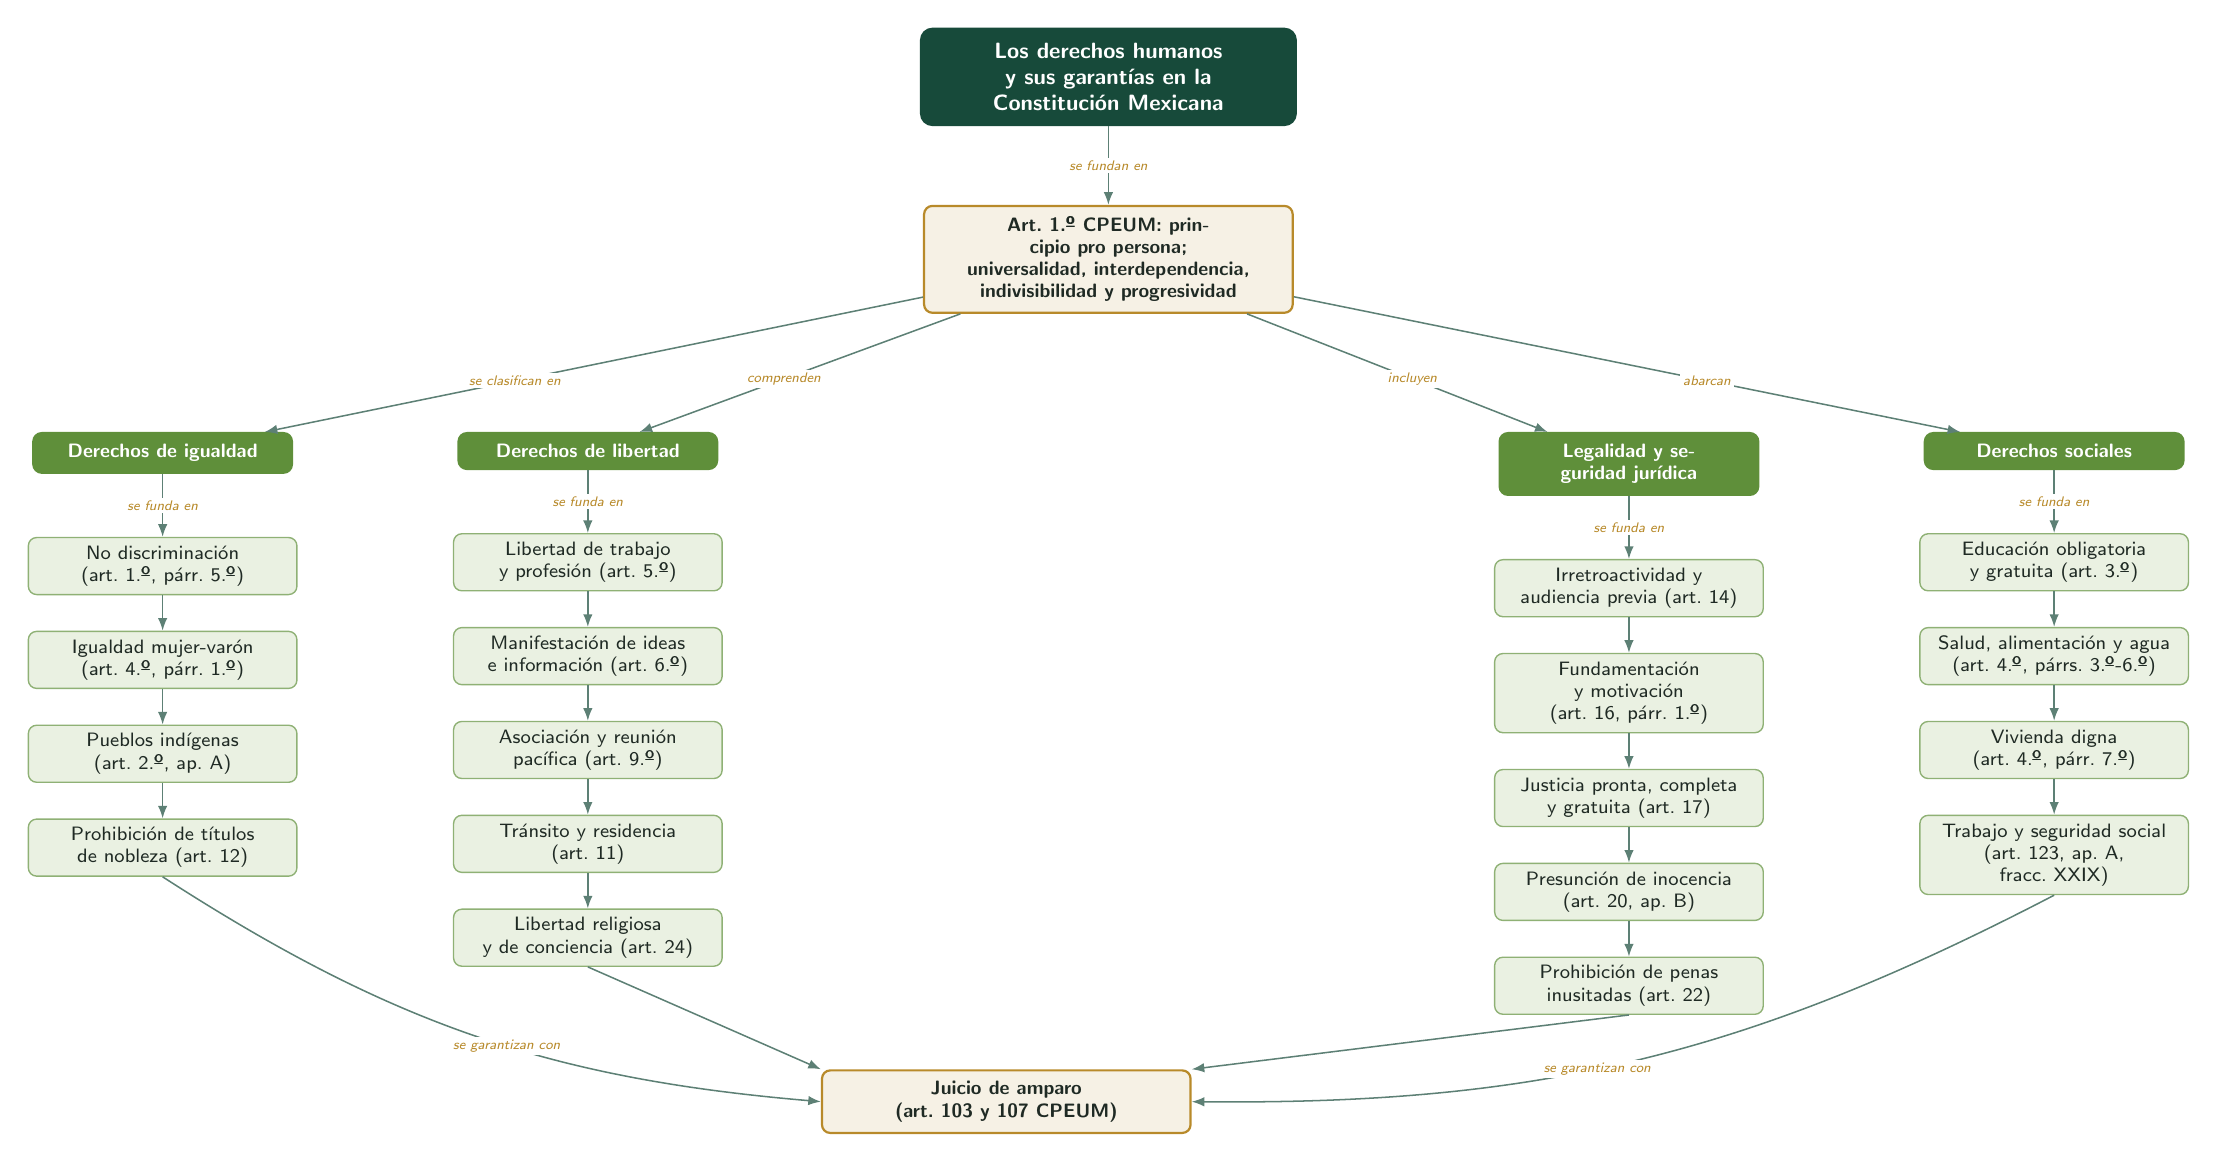
\begin{tikzpicture}[node distance=0.55cm and 0.9cm]

% ---- TEMA CENTRAL ----
\node[msroot] (root) {Los derechos humanos y sus garantías en la Constitución Mexicana};

% ---- NORMA DE APERTURA ----
\node[msnorm, below=1.0cm of root] (base) {Art.~1.º CPEUM: principio pro persona;\\ universalidad, interdependencia,\\ indivisibilidad y progresividad};
\draw[mslink] (root) -- node[mslabel]{se fundan en} (base);

% ---- CAMPOS SEMÁNTICOS (abanico radial) ----
\node[msfield, below left=1.5cm and 8.0cm of base] (c1) {Derechos de igualdad};
\node[msfield, below left=1.5cm and 2.6cm of base] (c2) {Derechos de libertad};
\node[msfield, below right=1.5cm and 2.6cm of base] (c3) {Legalidad y seguridad jurídica};
\node[msfield, below right=1.5cm and 8.0cm of base] (c4) {Derechos sociales};

\draw[mslink] (base) -- node[mslabel,pos=0.62]{se clasifican en} (c1);
\draw[mslink] (base) -- node[mslabel,pos=0.55]{comprenden} (c2);
\draw[mslink] (base) -- node[mslabel,pos=0.55]{incluyen} (c3);
\draw[mslink] (base) -- node[mslabel,pos=0.62]{abarcan} (c4);

% ---- CAMPO 1: IGUALDAD ----
\node[msleaf, below=0.8cm of c1] (c1a) {No discriminación\\ (art.~1.º, párr.~5.º)};
\node[msleaf, below=0.45cm of c1a] (c1b) {Igualdad mujer-varón\\ (art.~4.º, párr.~1.º)};
\node[msleaf, below=0.45cm of c1b] (c1c) {Pueblos indígenas\\ (art.~2.º, ap.~A)};
\node[msleaf, below=0.45cm of c1c] (c1d) {Prohibición de títulos\\ de nobleza (art.~12)};
\draw[mslink] (c1) -- node[mslabel]{se funda en} (c1a);
\draw[mslink] (c1a) -- (c1b);
\draw[mslink] (c1b) -- (c1c);
\draw[mslink] (c1c) -- (c1d);

% ---- CAMPO 2: LIBERTAD ----
\node[msleaf, below=0.8cm of c2] (c2a) {Libertad de trabajo\\ y profesión (art.~5.º)};
\node[msleaf, below=0.45cm of c2a] (c2b) {Manifestación de ideas\\ e información (art.~6.º)};
\node[msleaf, below=0.45cm of c2b] (c2c) {Asociación y reunión\\ pacífica (art.~9.º)};
\node[msleaf, below=0.45cm of c2c] (c2d) {Tránsito y residencia\\ (art.~11)};
\node[msleaf, below=0.45cm of c2d] (c2e) {Libertad religiosa\\ y de conciencia (art.~24)};
\draw[mslink] (c2) -- node[mslabel]{se funda en} (c2a);
\draw[mslink] (c2a) -- (c2b);
\draw[mslink] (c2b) -- (c2c);
\draw[mslink] (c2c) -- (c2d);
\draw[mslink] (c2d) -- (c2e);

% ---- CAMPO 3: LEGALIDAD Y SEGURIDAD JURÍDICA ----
\node[msleaf, below=0.8cm of c3] (c3a) {Irretroactividad y\\ audiencia previa (art.~14)};
\node[msleaf, below=0.45cm of c3a] (c3b) {Fundamentación y motivación\\ (art.~16, párr.~1.º)};
\node[msleaf, below=0.45cm of c3b] (c3c) {Justicia pronta, completa\\ y gratuita (art.~17)};
\node[msleaf, below=0.45cm of c3c] (c3d) {Presunción de inocencia\\ (art.~20, ap.~B)};
\node[msleaf, below=0.45cm of c3d] (c3e) {Prohibición de penas\\ inusitadas (art.~22)};
\draw[mslink] (c3) -- node[mslabel]{se funda en} (c3a);
\draw[mslink] (c3a) -- (c3b);
\draw[mslink] (c3b) -- (c3c);
\draw[mslink] (c3c) -- (c3d);
\draw[mslink] (c3d) -- (c3e);

% ---- CAMPO 4: DERECHOS SOCIALES ----
\node[msleaf, below=0.8cm of c4] (c4a) {Educación obligatoria\\ y gratuita (art.~3.º)};
\node[msleaf, below=0.45cm of c4a] (c4b) {Salud, alimentación y agua\\ (art.~4.º, párrs.~3.º-6.º)};
\node[msleaf, below=0.45cm of c4b] (c4c) {Vivienda digna\\ (art.~4.º, párr.~7.º)};
\node[msleaf, below=0.45cm of c4c] (c4d) {Trabajo y seguridad social\\ (art.~123, ap.~A, fracc.~XXIX)};
\draw[mslink] (c4) -- node[mslabel]{se funda en} (c4a);
\draw[mslink] (c4a) -- (c4b);
\draw[mslink] (c4b) -- (c4c);
\draw[mslink] (c4c) -- (c4d);

% ---- CIERRE DEL SISTEMA: MEDIO DE CONTROL ----
\node[msnorm, below=1.3cm of c2e.south east, xshift=3.6cm] (amparo) {Juicio de amparo\\ (art.~103 y 107 CPEUM)};
\draw[mslink] (c1d.south) to[bend right=14] node[mslabel,pos=0.55]{se garantizan con} (amparo.west);
\draw[mslink] (c4d.south) to[bend left=14] node[mslabel,pos=0.55]{se garantizan con} (amparo.east);
\draw[mslink] (c2e.south) -- (amparo.north west);
\draw[mslink] (c3e.south) -- (amparo.north east);

\end{tikzpicture}}
\end{center}

\captionof{figure}{Mapa semántico de los derechos humanos y sus garantías en la Constitución Política de los Estados Unidos Mexicanos. Elaboración propia con fundamento en el texto constitucional vigente \citep{cpeum2026}.}

\end{landscape}

\subsection{Del artículo 1.º al juicio de amparo: recorrido del mapa}

El mapa se lee de arriba hacia abajo. El tema central se apoya en el artículo 1.º constitucional, que opera como norma de apertura: reconoce los derechos previstos en la Constitución y en los tratados internacionales, incorpora el principio pro persona y fija los cuatro principios rectores del sistema \citep{cpeum2026}. Ese nodo explica por qué los cuatro campos comparten un mismo fundamento y no constituyen catálogos independientes.

Los campos se despliegan en abanico. El de \textbf{igualdad} reúne los preceptos que prohíben distinciones arbitrarias, desde la cláusula antidiscriminatoria hasta la prohibición de títulos de nobleza. El de \textbf{libertad} agrupa las esferas de autonomía personal que la autoridad no puede invadir sin fundamento expreso. El de \textbf{legalidad y seguridad jurídica} concentra las garantías procesales que someten al poder público a reglas conocidas de antemano. El de \textbf{derechos sociales} reúne las prestaciones que exigen del Estado una conducta activa \citep{cndhCualesDerechos2026}.

\textbf{Sin embargo}, la diferencia decisiva entre campos no radica en su importancia sino en el tipo de obligación que generan. Los tres primeros se satisfacen principalmente con abstenciones y con el respeto al procedimiento; \textbf{en cambio}, el cuarto exige organizar servicios y destinar recursos, \textbf{por consiguiente} su garantía es progresiva y queda sujeta al principio de no regresión \citep{alvarezIcazaDerechosMexico}.

Las palabras enlace hacen explícita cada relación. Los conectores \emph{se clasifican en}, \emph{comprenden}, \emph{incluyen} y \emph{abarcan} indican que los campos derivan del fundamento común; \emph{se funda en} vincula cada campo con sus preceptos; y \emph{se garantizan con} conduce al juicio de amparo, que cierra el sistema al convertir el reconocimiento en pretensión procesalmente accionable \citep{marcanoSalazarDerechosHumanos}.

\clearpage
\section{Conclusión}

Construir este mapa semántico permitió comprobar una idea que la lectura lineal del texto constitucional oculta: los derechos humanos no forman un listado, sino un sistema donde cada prerrogativa se conecta con un fundamento normativo preciso y con un mecanismo de exigibilidad determinado. \textbf{Considero} que representar esa estructura de forma visual aporta algo que la prosa difícilmente logra, porque muestra al mismo tiempo la clasificación y las relaciones.

La exigencia de correlacionar cada concepto con su artículo, fracción o párrafo resultó el elemento más formativo del ejercicio, \textbf{puesto que} obliga a verificar el texto normativo en lugar de confiar en la memoria y revela imprecisiones que pasarían inadvertidas en una redacción general. \textbf{Por tanto}, el mapa no solo sintetiza: \textbf{además} funciona como instrumento de control sobre la propia comprensión del tema \citep{cndhInehrmArticulo1o2015}.

\textbf{Sostengo} que el nodo del juicio de amparo es el que da sentido al conjunto. Sin un medio de control constitucional accesible, los cuatro campos quedarían como declaraciones sin consecuencia jurídica. Al incorporarlo como cierre del mapa quise mostrar que la garantía no es un apéndice del derecho, sino la condición que lo vuelve operativo frente a la autoridad.\footnote{En la elaboración de este trabajo se utilizaron herramientas de inteligencia artificial como apoyo para la organización y revisión del texto, conforme a los Lineamientos para el uso ético y responsable de la Inteligencia Artificial en el ámbito académico de la UnADM. La selección de conceptos, la verificación de los fundamentos constitucionales, el diseño del mapa y la postura sostenida son de mi autoría.}

\clearpage
\bibliography{garantias-constitucionales}

\end{document}
